\chapter{Methods}
\label{ch:whatYouDid}

\com{
\todo[inline]{Choose your own chapter title to describe this}

\todo[inline]{What have you done? How did you do it? What design decisions did you make? How did what you did help you to meet your goals?}



Describe the engineering-related contents (preferably with models) and the research methodology and methods that are used in the degree project. 

Give a theoretical description of the scientific or engineering methodology are you going to use and why have you chosen this method. What other methods did you consider and why did you reject them.

In this chapter, you describe what engineering-related and scientific skills you are going to apply, such as modeling, analyzing, developing, and evaluating engineering-related and scientific content. The choice of these methods should be appropriate for the problem . Additionally, you should be consciousness of aspects relating to society and ethics (if applicable). The choices should also reflect your goals and what you (or someone else) should be able to do as a result of your solution - which could not be done well before you started.

The purpose of this chapter is to provide an overview of the research method
used in this thesis. Section~\ref{sec:researchProcess} describes the research
process. Section~\ref{sec:researchParadigm} details the research
paradigm. Section~\ref{sec:dataCollection} focuses on the data collection
techniques used for this research. Section~\ref{sec:experimentalDesign}
describes the experimental design. Section~\ref{sec:assessingReliability}
explains the techniques used to evaluate the reliability and validity of the
data collected. Section~\ref{sec:plannedDataAnalysis} describes the method
used for the data analysis. Finally, Section~\ref{sec:evaluationFramework}
describes the framework selected to evaluate xxx.

}

\section{Research Methodology}
During this degree project, the research methodology\cite{RESEARCHMETHOD} will follow a quantitative approach: acquiring measurements and using them to validate or not the formulated research questions through quantitative analysis. 
The assumptions will follow an objective and realistic paradigm where the final results will be evinced quantifying measures of the observations and gaining a better knowledge of the environment.
The research method adopted will be experimental to understand the cause and effect of the obtained measurements, improving where possible, and descriptive to analyse the characteristics of the obtained system.
A deductive approach will be used to test the theories and draw conclusions about the hypotheses described in the research questions.
The research strategy adopted will be based on data collection through multiple case studies of experimental nature and the collected data will be analysed with computational mathematics. Statistical analysis will be used to test the quality of the obtained results. In particular, in this degree project, I will apply and discuss the validity, reliability, replicability, and ethics of those results.

The steps required for the fulfillment of this project are the following:
\begin{itemize}
    \item Analysis of available platform: the documentation made available by the \gls{HRP} and by the previous thesis student is studied to gain a more comprehensive understanding of the automower implementation.
    \item Analysis of the state-of-the-art: a research on possible improvements to be investigated is performed, addressing unsolved issues found in the previous step.
    \item Implementation of identified approach: after the initial phase of identification of the topic, the system will be expanded and improved upon with the selected features described above.
    \item Testing of the obtained system: during this phase, it will be important to continuously test the upgrades with multiple tests, allowing for a robust analysis of the specified additions.
    \item Improvement upon found vulnerabilities: the problems and inaccuracies that will eventually come up during the testing phase will be investigated and eventually fixed to provide a overall more reliable system. 
\end{itemize}

Finally, to evaluate if the objectives have been fulfilled and the results can be evaluated as valuable, the following steps are required:
\begin{itemize}
    \item The quantitative measures need to be tested in a real use case experiment, as specified in the research questions.
    \item The data, acquired during these testing phases, will be used and analysed to check if the set of objectives have been reached.
    \item A statistical analysis over multiple experimental tests will provide more reliable results to be presented in the final report.
\end{itemize}



To gather data used to test and analyse the performance of the system, multiple outdoor tests have been carried on.
Some tests have been made to define the calibration of the sensors against a ground truth identified using measure tape. 
Some other tests have been made to ensure that the system is behaving accurately while steering.
Some tests have been made to check that the collision events are estimated with an certain degree of precision.

During these tests the rosbag utils provided by ROS has been exploited. Through this service it is possible to store every message sent to the topics, and they can be reused in the future to tune the algorithms.
In this way, the real measurements gathered during outdoor testing can be re evaluated through the play of said messages and using a simulated parameter to reset the clock of ROS framework.


\section{System Configuration}
\label{sec:system}

\noindent 
Raspberry Pi 4 to guide the automower, to gather information about the topics of ROS, and to communicate them to the personal computer used to gather them.
Husqvarna Automower that holds the sensors and the raspberry pi, also proving the measurements of the wheel encoders and of the embedded GPS receiver. 
Computer to guide the automower and make him move according to the desired path, also at the end the automower was free to run its random path and use the algorithm implemented to stay inside the boundaries.
 
\com{
\begin{figure}[!ht]
  \begin{center}
    \includegraphics[width=0.5\textwidth]{Images/4-Done/}
  \end{center}
  \caption{Hardware}
  \label{fig:hardware}
\end{figure}
}


\subsection{Mobile Robots}

\noindent Mobile robots are robotics systems which are able to move themselves on the environment they are in. 
The outdoor mobile robotics platform used for the purpose of this thesis is the \gls{HRP}.
It is a \Gls{ROS}-enabled and adapted wheeled mobile robot used to mow the lawn in an autonomous manner.
It will be used as base to implement the additional sensors, to experiment their configuration, and to test their performances.
An analysis of the kinematic model of this \Gls{UGV} is firstly presented here, followed by an overview of the \gls{ROS} framework.

For the scope of this thesis, just the kinematics have been considered as other aspects, such as torque, friction, physical implications, and in general the dynamics of the systems, are not relevant to be analysed.


\subsection{Kinematic Model}

\noindent The mobile robot used equips two standard back wheels with differential drive, and two castor wheels on the front, which allow free rotation around the wheel axle for multiple direction steering. It can be seen in figure \ref{fig:kine}
It is propelled by two separate motors mounted along the axis of the back wheels, thus the movements of the robot are made by controlling each back wheel velocity individually.

\begin{figure}[!ht]
%\textbf{Investigating Simultaneous Localization and Mapping for AGV systems} 
  \begin{center}
    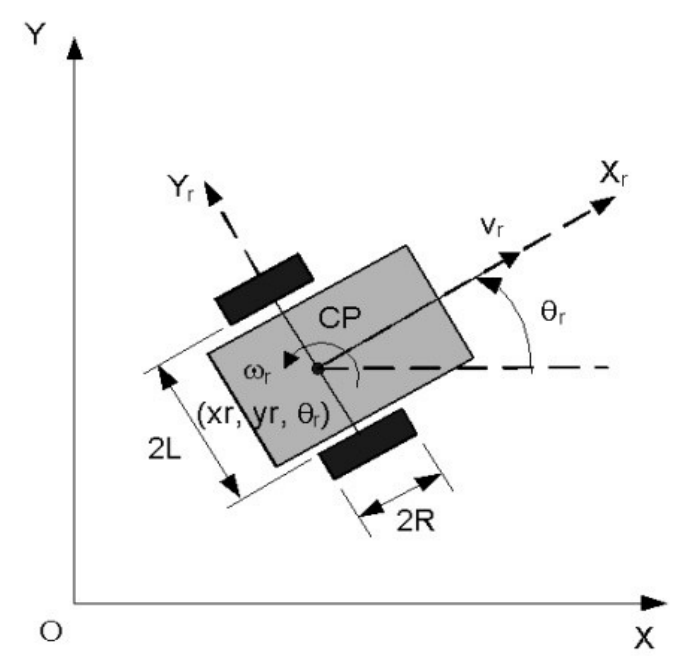
\includegraphics[width=0.75\textwidth]{Images/2-Background/Kinematics-2021-04-23 13-55-11.png}
  \end{center}
  \caption{Kinematic model of a differential drive mobile robot \cite{trajectory}.}
  \label{fig:kine}
\end{figure}

This differential drive system is not able to freely move along the \gls{2D} environment, as the degrees of freedom, defined by $\begin{bmatrix}x&y&\theta\end{bmatrix}$, are less than the degrees of mobility, given by the wheels velocities $\begin{bmatrix}\dot \delta _L & \dot \delta _R\end{bmatrix}$.
The system is thus called non-holonomic and a non-holonomic constraint has to be defined.
The standard wheels used by the differential mobile robot are subject to such non-holonomic rolling constraint, which limits the sideways sliding by imposing that the wheel spins purely along the direction of the wheel.
Non-holonomic constraints do not allow for integration of the differential equations to retrieve the final pose, since the displacements of each wheel are not sufficient to determine it.
This forces the position and orientation to be estimated using integration of wheels velocities rather than their position displacements.
However, with a sufficient sampling rate, an integrable approach can be used to estimate its pose, but the usage of incremental displacements provided by integration of velocity measurements will inevitably accumulate errors over time.


\subsubsection{Forwards Kinematics}
\label{sec:forwards}

Through the usage of wheel encoders attached to both these wheels, an estimated velocity for them is calculated and used to determine its pose.
This open-loop technique to determine the position and orientation is called \gls{DR}, as the new pose is estimated by using the last known pose and the new speed measurements.

The wheel encoders attached on each wheel provide an estimate of the number of pulses they detected. These encoder pulses need to be translated to an approximated wheel displacement through the transformation constant $C_{D}$ provided by equation \ref{eq:wheel_meter}.
\begin{equation}
C_{D} = \frac{\pi \cdot W_D }{E_T}
\label{eq:wheel_meter}
\end{equation} where $W_D$ is the estimated length of the wheel diameter and $E_T$ is the encoder time resolution.
This value is used to derive the velocity of each wheel separately, $\dot \delta_L$ and $\dot \delta_R$, by multiplying their encoder pulses, $E_L$ and  $E_R$ respectively, with transformation constant and dividing it using the time delay $\Delta_t$, as in equation \ref{eq:wheel_disp}.
\begin{equation}
\dot \delta_{L} = \frac{C_D \cdot E_L}{\Delta_t}  \qquad
\dot \delta_{R} = \frac{C_D \cdot E_R}{\Delta_t}
\label{eq:wheel_disp}
\end{equation}

Using these single wheel displacements, it is possible to calculate the linear velocity along the $x$ axis, $v$, and the angular velocity on the $z$ axis, $\omega$, with respect to the mobile robot frame using equations \ref{eq:disp}:
\begin{equation}
    v =\frac{\dot \delta_{R} + \dot \delta_{L} }{2} \qquad \omega = \frac{\dot \delta _{R} - \dot \delta_{L}}{B_W}
\label{eq:disp}
\end{equation} where $B_W$ is the estimated length of the base width of the back wheel axis.


These forward kinematics equations of this differential drive mobile robot are used to update the pose of the mobile robot, from time $t$ after a time step $\Delta_t$ to time $t+1$, in the global coordinate frame with the Euler first-order differential approximation~\cite{braun_first-order_1993}, as shown in equation \ref{eq:euler}.

\begin{equation}
\begin{bmatrix} x_{t + 1} \\ y_{t + 1} \\ \theta _{t + 1} ~ \end{bmatrix}
= 
\begin{bmatrix} {x_t} \\ {y_t} \\ {\theta _t}  \end{bmatrix} 
+ 
\begin{bmatrix}  \cos (\theta _t ) & 0\\  \sin (\theta _t ) & 0 \\ 0 & 1 \end{bmatrix}
\cdot 
\begin{bmatrix} v \\ \omega \end{bmatrix} \cdot
\Delta_t
\label{eq:euler}
\end{equation}


This method however is subject to multiple errors and inaccuracies, as the measurements and time delays will never be perfect. 
The systematic errors can be given by imperfectness of robot model as impreciseness in the wheel diameters or wheel base measures, which are used to estimate the movements. 
However, the presence of non-systematic random errors as result of usage of imperfect measurements are more difficult to model, e.g. wheel slippage, uneven terrain, and external forces applied.
The accumulative characteristic of these errors will break the stability of the system, making the estimate to drift after a period of time.
These conditions render this \gls{DR} model not adequate to determine the pose of the mobile robot, but its estimate could be used anyway to improve the positioning system. 


\subsubsection{Velocity Control}
\label{sec:control}
\noindent A script is used to control the vehicle setting the desired robot velocities: $v$ and $\omega$.
In this way it is possible to command the \gls{ALM} to follow a trajectory.

\subsection{Robotic Operating System}

\noindent \Gls{ROS}\cite{288} is an open-source framework, and not an actual operating system, widely adopted for building software used to control robotic systems.
\Gls{ROS} works both with C++ and Python programmed scripts, allowing for developers with different backgrounds to develop upon it.

During the past decade it has seen numerous improvements by the community and it provides a collection of several libraries, tools, and conventions made to simplify the modular creation and interaction of complex robotic systems.
Its modular structure is composed by available packages containing well-debugged code which can be adapted and run together with newly made packages built to satisfy the projects requirements.
These packages are composed by modules of software which can be described as custom nodes, libraries, processes, and messages.
A robotic system operates using an interconnection of different nodes which have just minimal tasks to execute.
Its services are mostly developed as a middle-layer infrastructure to allow for interaction of heterogeneous devices, ranging from low-level device control to embedded system, providing hardware abstraction and enabling message-passing between processes.

For these nodes to cooperate, they are connected by a middle-layer structure based on a network of topics or services, following a blackboard architecture of data sharing.
It provides a graph-like structure were each program, described as node, can both publish and subscribe messages among the created and available topics.
Topics can be seen as variables which are used for streaming communication and share information between nodes. 
A \Gls{ROS} node publishes a specific message through a topic and every other node can subscribe to that topic and receive all the messages posted to it.
A \Gls{ROS} system, to behave as expected, needs a master process which has the task of matching publishers and subscribers to their related topics.
These topics can be generated by sensors, actuators, planners, controllers of different kind and made available using this structure of topics, similar to a blackboard architecture.
Each topic is defined by a specific message type which specifies its content in order to standardise its usage among applications and to simplify communication between nodes. 
Messages definition can be customised and they are stored inside the \Gls{ROS} package, defining the data sent within the topic which will use that definition.
Figure \ref{fig:ros-topic} shows an example of a \Gls{ROS} graph where two subscriber nodes receive the messages posted on the topic by a publisher node.
    
\begin{figure}[!ht]
%\textbf{Investigating Simultaneous Localization and Mapping for AGV systems} 
  \begin{center}
    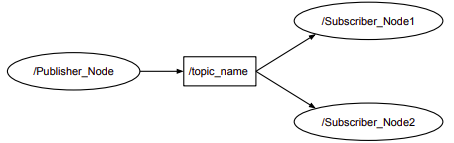
\includegraphics[width=0.75\textwidth]{Images/2-Background/ROSTopic-2021-04-22 10-51-37.png}
  \end{center}
  \caption{Example of \Gls{ROS} architecture for information sharing\cite{palsson_investigating_2017}}
  \label{fig:ros-topic}
\end{figure}

The aspect of localisation is important for the robotics field, to understand where the robot is located with respect to the rest of the world, but also to know how the sensors are positioned with respect to the robot in which they are installed.
It is of prominent importance to be aware of the different pose of the connected sensors before fusing their information, as the measurements of each sensors are related to their specific coordinate frame.
Before performing sensors fusion, every different frames of the sensors need to be transformed into the base frame of the robot which they are measuring to be sure about that the measurements refers to the same coordinate frame. 
\Gls{ROS} uses the TF\cite{6556373} library to provide the tools needed to work with coordinate frames and to deal with their related transformation.
It allows for the definition of each sensor rigid body transform to specify their related position with respect to the robot, and then the library will deal with all the other transformations by publishing messages regarding to the rotational and translational relations between frames.
Commonly used frames are odom and base\_link, as shown in figure \ref{fig:ros-frames}. The odom frame has the origin at the initial position $P_{odom}$ of the robot and it is used to keep track of its moving behaviour. The base\_link frame is rigidly attached to the robot base $P_{base}$ and it is used to define the frames of its attached components. A transformation to map the the base\_link frame into the odom frame in \Gls{2D} with a rotation along the Z axis of $\theta$ and with a translation of $(x',y')$ is defined using an orthogonal matrix as in equation \ref{eq:transf}:
\begin{align}
P_{odom} = T^o_b \cdot P_{base} && \textrm{where} ~ 
T^o_b = 
\begin{bmatrix}
cos(\theta) & -sin(\theta) & x' \\
sin(\theta) & cos(\theta) & y' \\
0 & 0 & 1 \\
\end{bmatrix} 
\label{eq:transf}
\end{align}


\begin{figure}[!ht]
%\textbf{Investigating Simultaneous Localization and Mapping for AGV systems} 
\begin{center}
    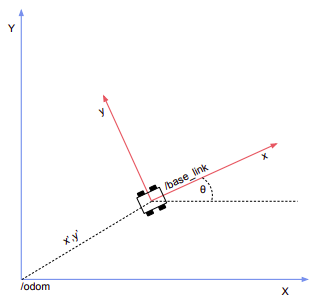
\includegraphics[width=0.5\textwidth]{Images/2-Background/Frames-2021-04-22 12-03-22.png}
  \end{center}
  \caption{Example of relation between \Gls{ROS} frames.\cite{palsson_investigating_2017}}
  \label{fig:ros-frames}
\end{figure}
    


\subsection{Kinematics}
\label{ssec:dev}
\noindent 
Model

Forward kinematics

\subsection{Devices}
\label{ssec:dev}
\noindent 


\subsubsection{Raspberry Pi 4}
\noindent 


\subsubsection{Raspberry Pi 3}
\noindent 


\subsection{Sensors}
\label{ssec:sens}
\noindent 

\subsubsection{Wheel Encoder}
\noindent 

\subsubsection{Global Navigation System S}
\noindent 

\subsubsection{IMU}
\noindent 


\subsubsection{Camera}
\noindent Using the \gls{RTABMAP} package\footnote{\url{http://introlab.github.io/rtabmap/}}\cite{6094602} \cite{labbe_rtab-map_2019}, more specifically the \gls{ROS} version 0.20.9 found on github for \gls{ROS} Noetic.



\subsection{Software Tools}
\noindent 
C++ and Python development to work with the ROS framework.

Network establishment to communicate wirelessly between Raspberry Pi and computer.

Communication through hotspot 


\subsection{Robotic Operating System configuration}
\label{ssec:ros}
\noindent 
Executing automower\_hrp.launch

Executing hrp\_teleop.launch

Executing imus\_basic.launch

Executing gps.launch

Executing rs\_camera.launch

Executing VO package

Executing EKF

Executing map generation and update





 
\section{Localisation Configuration}
\label{sec:locConf}
%\begin{figure}[!ht]
%  \begin{center}
%    \includegraphics[width=0.25\textwidth]{Homepage-icon.png}
%  \end{center}
%  \caption{Homepage icon}
%  \label{fig:homepageicon}
%\end{figure}


\subsection{ \gls{EKF} Prediction}

\noindent 
As we are working in 2D, the state variables needed are the following:
$$
  \label{eq:state-transf}
\mathbf{X}_t=
\begin{bmatrix} 
\mathbf{x}_t & \mathbf{y}_t & \boldsymbol \theta_t & \mathbf{v}_t & \dot{\boldsymbol \omega}_t & \mathbf{a}_t 
\end{bmatrix} ^T
$$

\subsubsection{Transition}

\noindent 
\begin{equation}
A_t
=
\begin{bmatrix} 
1 & 0 & 0 & \cos(\boldsymbol \theta_t) \cdot \Delta_t & 0 & \cos(\boldsymbol \theta_t) \cdot  \cfrac{\Delta_t^2 }{2} \\ 
0 & 1 & 0 & \sin(\boldsymbol \theta_t) \cdot \Delta_t & 0 & \sin(\boldsymbol \theta_t) \cdot  \cfrac{\Delta_t^2 }{2} \\ 
0 & 0 & 1 & 0 & \Delta_t & 0 \\ 
0 & 0 & 0 & 1 & 0 & \Delta_t \\ 
0 & 0 & 0 & 0 & 1 & 0 \\ 
0 & 0 & 0 & 0 & 0 & 1 
\end{bmatrix}
\end{equation}


\subsubsection{Control}

\noindent 
\begin{align}
B
= 
    \begin{bmatrix} 
    0 & 0 \\
    0 & 0\\
    0 & 0\\
    s_v & 0\\
    0 & s_{ \dot{\boldsymbol \theta}}\\
    0 & 0\\
    0 & 0 
    \end{bmatrix}
& \quad
\mathbf{u}_t
= 
    \begin{bmatrix} 
    \boldsymbol \Delta_{\mathbf{v}}  \\
    \boldsymbol \Delta_{ \dot{\boldsymbol \theta}} \\[0.3em]
    \end{bmatrix}
\end{align}
where:
  \begin{align}
     \boldsymbol \Delta_{\mathbf{v}} = \text{Control}_{\mathbf{v}} - \mathbf{v}_t  \\
    \boldsymbol \Delta_{ \dot{\boldsymbol \theta}} = \text{Control}_{\dot{\boldsymbol \theta}} - \dot{\boldsymbol \theta}_t
  \end{align}
$ \text{Control}_{\mathbf{v}}$ and  $\text{Control}_{\mathbf{\dot{\boldsymbol \theta}}}$ are the command sent to the robot, obtained by a specific topic.

$s_{.}$ instead is used to make the transition from command received and actual actuation more smooth by limiting the innovation given by the respective control through a scaling value $s_. = 0.5$


\subsubsection{Noise}

\noindent 
The noise vector is defined as
\begin{equation}
\boldsymbol \omega
=
\begin{bmatrix} 
\omega_{\mathbf{x}}  & 
\omega_{\mathbf{y}} &
\omega_{\boldsymbol \theta}  & 
\omega_{\mathbf{v}} & 
\omega_{\dot{\boldsymbol \theta}} &
\omega_{\mathbf{a}}
\end{bmatrix} ^T
\end{equation}
where $\omega_i \sim \mathcal{N}(\mu_i,\,\sigma_{ii}^{2})$ with $\mu_i = 0$, $\sigma_{ii}^2 = 0.1$, and $ i = \{ \mathbf{x} , \mathbf{y} , \boldsymbol \theta , \mathbf{v} , \mathbf{\dot{\boldsymbol \theta}} , \mathbf{a} \}$

The prediction step for the state variables is then the following
\begin{equation}
\mathbf{X}_{p} = A \cdot \mathbf{X}_t + B \cdot \mathbf{u}_t + \boldsymbol \omega
\end{equation}

Since we are dealing with an Extended Kalman Filter, the Jacobian of the transition matrix must be obtained to linearise the non-linear equations with a first order taylor expansion, obtaining :

\begin{equation}
J_A
=
\begin{bmatrix} 

1 & 0 & 0 & -\sin(\boldsymbol \theta_t) \cdot \Delta_t & 0 & -\sin(\boldsymbol \theta_t) \cdot  \frac{\Delta_t^2 }{2} \\ 
0 & 1 & 0 & \cos(\boldsymbol \theta_t) \cdot \Delta_t & 0 & \cos(\boldsymbol \theta_t) \cdot  \frac{\Delta_t^2 }{2} \\ 
0 & 0 & 1 & 0 & \Delta_t & 0 \\ 
0 & 0 & 0 & 1 & 0 & \Delta_t \\ 
0 & 0 & 0 & 0 & 1 & 0 \\ 
0 & 0 & 0 & 0 & 0 & 1 
\end{bmatrix}
\end{equation}

\begin{equation}
Q
=
\begin{bmatrix} 
\sigma_{\mathbf{xx}}^2 & 0 & 0 & 0 & 0 & 0 \\ 
0 & \sigma_{\mathbf{yy}}^2 & 0 & 0 & 0 & 0 \\ 
0 & 0 & \sigma_{\mathbf{\boldsymbol \theta \boldsymbol \theta}}^2 & 0 & 0 & 0 \\ 
0 & 0 & 0 & \sigma_{\mathbf{vv}}^2 & 0 & 0 \\ 
0 & 0 & 0 & 0 & \sigma_{\mathbf{\dot{\boldsymbol \theta}\dot{\boldsymbol \theta}}}^2 & 0 \\ 
0 & 0 & 0 & 0 & 0 & \sigma_{\mathbf{aa}}^2 \\ 
\end{bmatrix}
\end{equation}

Finally the covariance matrix after prediction is:

\begin{align}
    P_{p} & = J_A \cdot P_t \cdot J_A^T + Q && \\
    %P_{p} & =  \frac{P_{p} +  P_{p}^T}{2} && \text{To ensure symmetry} 
\end{align}


\subsection{Measurement Models}
\noindent Check for new measurements in background and dynamically create the components for the update step


\subsubsection{Wheel Encoder}

\noindent 
After the derivation of $\mathbf{v}$ and $\boldsymbol \omega$ as defined in equation \ref{eq:disp} in Section \ref{sec:forwards}:

Through the usage of wheel encoders attached to both these wheels, an estimated velocity for them is calculated and used to determine its pose.
This open-loop technique to determine the position and orientation is called \gls{DR}, as the new pose is estimated by using the last known pose and the new speed measurements.

The wheel encoders attached on each wheel provide an estimate of the number of pulses they detected. These encoder pulses need to be translated to an approximated wheel displacement through the transformation constant $C_{D}$ provided by equation \ref{eq:wheel_meter}.
\begin{equation}
C_{D} = \frac{\pi \cdot W_D }{E_T}
\label{eq:wheel_meter}
\end{equation} where $W_D$ is the estimated length of the wheel diameter and $E_T$ is the encoder time resolution.
This value is used to derive the velocity of each wheel separately, $\dot \delta_L$ and $\dot \delta_R$, by multiplying their encoder pulses, $E_L$ and  $E_R$ respectively, with transformation constant and dividing it using the time delay $\Delta_t$, as in equation \ref{eq:wheel_disp}.
\begin{equation}
\dot \delta_{L} = \frac{C_D \cdot E_L}{\Delta_t}  \qquad
\dot \delta_{R} = \frac{C_D \cdot E_R}{\Delta_t}
\label{eq:wheel_disp}
\end{equation}

Using these single wheel displacements, it is possible to calculate the linear velocity along the $x$ axis, $v$, and the angular velocity on the $z$ axis, $\omega$, with respect to the mobile robot frame using equations \ref{eq:disp}:
\begin{equation}
    v =\frac{\dot \delta_{R} + \dot \delta_{L} }{2} \qquad \omega = \frac{\dot \delta _{R} - \dot \delta_{L}}{B_W}
\label{eq:disp}
\end{equation} where $B_W$ is the estimated length of the base width of the back wheel axis.


These forward kinematics equations of this differential drive mobile robot are used to update the pose of the mobile robot, from time $t$ after a time step $\Delta_t$ to time $t+1$, in the global coordinate frame with the Euler first-order differential approximation~\cite{braun_first-order_1993}, as shown in equation \ref{eq:eulerWheel}.

\begin{equation}
\begin{bmatrix} x_{t + 1} \\ y_{t + 1} \\ \theta _{t + 1} ~ \end{bmatrix}
= 
\begin{bmatrix} {x_t} \\ {y_t} \\ {\theta _t}  \end{bmatrix} 
+ 
\begin{bmatrix}  \cos (\theta _t ) & 0\\  \sin (\theta _t ) & 0 \\ 0 & 1 \end{bmatrix}
\cdot 
\begin{bmatrix} v \\ \omega \end{bmatrix} \cdot
\Delta_t
\label{eq:eulerWheel}
\end{equation}


This method however is subject to multiple errors and inaccuracies, as the measurements and time delays will never be perfect. 
The systematic errors can be given by imperfectness of robot model as impreciseness in the wheel diameters or wheel base measures, which are used to estimate the movements. 
However, the presence of non-systematic random errors as result of usage of imperfect measurements are more difficult to model, e.g. wheel slippage, uneven terrain, and external forces applied.
The accumulative characteristic of these errors will break the stability of the system, making the estimate to drift after a period of time.
These conditions render this \gls{DR} model not adequate to determine the pose of the mobile robot, but its estimate could be used anyway to improve the positioning system. 




\begin{align}
\mathbf{v}_{Enc_t} & = \mathbf{v}\\
\boldsymbol \omega_{Enc_t} & = \boldsymbol \omega
\end{align}


Measurements vector with uncertainty vector
\begin{align}
\mathbf{Z}
=
\begin{bmatrix} 
\mathbf{v}_{Enc_t} \\
\boldsymbol \omega_{Enc_t} 
\end{bmatrix}^T
& \quad
\mathbf{R}
=
\begin{bmatrix} 
\eta_{\mathbf{v}_{Enc}} \\ 
\eta_{\boldsymbol \omega} 
\end{bmatrix}^T
\end{align}
where $ \omega_{\mathbf{x}_{Enc}} = \omega_{\mathbf{y}_{Enc}} = 1$ and 
$ \omega_{\boldsymbol \theta_{Enc}} = \pi/180 $ , experimentally derived.


Measurement Matrix
\begin{equation}
H
=
\begin{bmatrix} 
0 & 0 & 0 & 1 & 0 & 0 \\ 
0 & 0 & 0 & 0 & 1 & 0
\end{bmatrix}
\end{equation}

Measurement Jacobian Matrix
\begin{equation}
J_H
=
\begin{bmatrix} 
0 & 0 & 0 & 1 & 0 & 0 \\ 
0 & 0 & 0 & 0 & 1 & 0
\end{bmatrix}
\end{equation}


\subsubsection{GPS}

\noindent In order to get the mean using the first measurements before the first command to move the automower, those values are stored in $\mu_{lat}$ and $\mu_{long}$.

The formula used to obtain the distance between this mean value and the current value of the gps measurements can be found at Appendix

\begin{align}
\mathbf{x}_{GPS_t} & = \text{geodetic2enu}( z_{lat} - \mu_{lat})\\
\mathbf{y}_{GPS_t} & = \text{geodetic2enu}( z_{long} - \mu_{long})
\end{align}



\begin{equation}
z_{\boldsymbol \theta_{GPS_t}} = \arctan(\mathbf{y}_{GPS_{t-1}} - \mathbf{y}_{GPS_t}, \mathbf{x}_{GPS_{t-1}} - \mathbf{x}_{GPS_t} )
\end{equation}

In this section we shall assume that wrapping operation
amounts to enforcing the angular variable to be in the [$-\pi$, $\pi$]
interval, and we designate this operation as follows
\begin{equation}
w_{\pi}(x) = mod(x + \pi, 2\pi) - \pi
\end{equation}

Note that when computing the difference between two angular
variables, the wrapping effect of the circle should be taken into
account, e.g., the difference between 178° and -178° should
evaluate to 4°. This is achieved by the function $w_{\pi}(x)$ when the difference
is given as the argument, i.e., difference between two angles
x and y is computed as $w_{\pi}(x-y)$, as defined in "On wrapping the Kalman filter and estimating with
the SO(2) group"

$$
\boldsymbol \theta_{GPS_t} = \boldsymbol \theta_{t} + w_{\pi}(z_{\boldsymbol \theta_{GPS_t}} - \boldsymbol \theta_{t})
$$

Measurements vector with uncertainty vector
\begin{align}
\mathbf{Z}
=
\begin{bmatrix} 
\mathbf{x}_{GPS_t} \\ 
\mathbf{y}_{GPS_t} \\ 
\boldsymbol \theta_{GPS_t} \\ 
\end{bmatrix}^T
& \quad
\mathbf{R}
=
\begin{bmatrix} 
\omega_{\mathbf{x}_{GPS}} \\ 
\omega_{\mathbf{y}_{GPS}} \\ 
\omega_{\boldsymbol \theta_{GPS}} \\ 
\end{bmatrix}^T
\end{align}
where $ \omega_{\mathbf{x}_{GPS}} = \omega_{\mathbf{y}_{GPS}} = \text{HDOP} = \sqrt{\sigma_x^2 + \sigma_y^2}$ and 
$ \omega_{\boldsymbol \theta_{GPS}} = \pi/8 $ , experimentally derived.

Measurement Matrix
\begin{equation}
H
=
\begin{bmatrix} 
1 & 0 & 0 & 0 & 0 & 0 \\ 
0 & 1 & 0 & 0 & 0 & 0 \\ 
0 & 0 & 1 & 0 & 0 & 0 \\ 
\end{bmatrix}
\end{equation}

Measurement Jacobian Matrix
\begin{equation}
J_H
=
\begin{bmatrix} 
1 & 0 & 0 & 0 & 0 & 0 \\ 
0 & 1 & 0 & 0 & 0 & 0 \\ 
0 & 0 & 1 & 0 & 0 & 0 \\ 
\end{bmatrix}
\end{equation}



\subsubsection{IMU}

\noindent 
Measurements vector, as obtained by IMU, with uncertainty vector
\begin{align}
\mathbf{Z}
=
\begin{bmatrix} 
\dot{\boldsymbol \theta }_{IMU_t} \\ 
\mathbf{a}_{IMU_t} \\ 
\end{bmatrix}^T
& \quad
\mathbf{R}
=
\begin{bmatrix} 
\omega_{\dot{\boldsymbol \theta}_{IMU}} \\ 
\omega_{\mathbf{a}_{IMU}} \\ 
\end{bmatrix}^T
\end{align}
where $ \omega_{\dot{\boldsymbol \theta}_{IMU}} = 1$ and 
$ \omega_{\mathbf{a}_{IMU}} = 4 $ , experimentally derived.


Measurement Matrix
\begin{equation}
H
=
\begin{bmatrix} 
0 & 0 & 0 & 0 & 1 & 0 \\ 
0 & 0 & 0 & 0 & 0 & 1 \\ 
\end{bmatrix}
\end{equation}

Measurement Jacobian Matrix
\begin{equation}
J_H
=
\begin{bmatrix} 
0 & 0 & 0 & 0 & 1 & 0 \\ 
0 & 0 & 0 & 0 & 0 & 1 \\ 
\end{bmatrix}
\end{equation}

\subsubsection{Visual Odometry}
\noindent 
Measurements vector, as obtained by the \gls{RTABMAP} package in \gls{ROS}.
It delivers only the velocities, as the position is drifting. Moreover, it also provides its own uncertainty vector error based on the uncertainty of the estimation over the images.

Measurements vector with uncertainty vector
\begin{align}
\mathbf{Z}
=
\begin{bmatrix} 
\mathbf{v}_{Vis_t} \\
\boldsymbol \omega_{Vis_t} 
\end{bmatrix}^T
& \quad
\mathbf{R}
=
\begin{bmatrix} 
\eta_{\mathbf{v}_{Vis}} \\ 
\eta_{\boldsymbol \omega_{Vis}} 
\end{bmatrix}^T
\end{align}
where $ \omega_{\mathbf{x}_{Vis}} = \omega_{\mathbf{y}_{Vis}} = 1$ and 
$ \omega_{\boldsymbol \theta_{Vis}} = \pi/180 $ , experimentally derived.


Measurement Matrix
\begin{equation}
H
=
\begin{bmatrix} 
0 & 0 & 0 & 1 & 0 & 0 \\ 
0 & 0 & 0 & 0 & 1 & 0
\end{bmatrix}
\end{equation}

Measurement Jacobian Matrix
\begin{equation}
J_H
=
\begin{bmatrix} 
0 & 0 & 0 & 1 & 0 & 0 \\ 
0 & 0 & 0 & 0 & 1 & 0
\end{bmatrix}
\end{equation}



\subsection{Batch \gls{EKF} Correction}

\noindent 
Gather all measurements and then use those combined measures for one single correction step

Use of locks to work with the same matrices


\com{
    \lstset{extendedchars=true}
    \begin{lstlisting}[language={Python}, caption={Batch EKF}, label=lst:programmes]
    #  Start node
    #  Subscribe to topics
    #  Update
    #  Get measures
    #  Correct
    #  Sleep
    
    
    
    
    
    def v1_get_programmes():
        global Verbose_Flag
        #
        # Use the KOPPS API to get the data
        # note that this returns XML
        url = "{0}/api/kopps/v1/programme".format(KOPPSbaseUrl)
        if Verbose_Flag:
            print("url: " + url)
        #
        r = requests.get(url)
        if Verbose_Flag:
            print("result of getting v1 programme: {}".format(r.text))
        #
        if r.status_code == requests.codes.ok:
            return r.text           # simply return the XML
        #
        return None
    \end{lstlisting}
}


\com{\subsection{Iterated \gls{EKF} Correction}
\noindent 
As soon as a measure arrives, correct using just that measure, one step at the time
}


 
\section{Mapping Configuration}
\label{sec:locConf}

\noindent The occupancy grid is defined using \gls{ROS}. It is composed by a grid of cells of dimension \SI{150}{m}~x~\SI{150}{m}, with the center positioned in the middle of this square at position (\SI{75}{m}~,~\SI{75}{m}), and with a resolution of \SI{0.1}{m}. In this way, it will be possible to manage an area of \SI{5000}{m^2} whichever the configuration of the lawn.

The external boundaries are defined as $-1$ values, and so if the automower finds itself close to or directly on a cell with a value of $-1$, it will change its orientation and continue on his tasks.
The rest of the cells are initialised with value $50$, meaning that the initial assumption is that the environment is uncertain and that there might be obstacles present within it.
The value of each cell then contains the probability that an object is present in that position, with those values being updated with \todo[inline, inlinewidth=4cm, noinlinepar]{Probability merging} in case of collision event detected by the \gls{ALM}.

At the first run of the automower, the estimated trajectory derived by the EKF will be used to set the corresponding boundary, i.e. by setting the cells it directly travelled through to $-1$. 

After this guided procedure, the automower will have an estimate of its environment configuration and a virtual boundary to delimit its operations.

After this phase of boundary definition, the \gls{ALM} is left free to roam on that area.
Even if it is defined with cells containing values of $0$, it might still



\section{Testing Configuration}

\todo[inline]{This should also show that you are aware of the social and ethical concerns that might be relevant to your data collection method.)}

\label{sec:testing}
\noindent Multiple tests are made. 
The teleoperation script available is used to control the mobile robot in velocity.
The measures obtained by an experiments are stored in \gls{ROS} bags which can be used later on to test the filter multiple times with the same experiment.

Different configurations that are going to be tested provide different observabilty performance for the AEKF filter.
observability

\subsection{Ground Truth Generation}
\label{sec:gt}


\noindent The ground truth is constructed manually by checking the actual path travelled by the robot with the usage of a meter. Setting the experiment and having the robot to follow that path manually, commanding it using the given teleoperation script.



\subsection{Simulation design}
\label{sec:simDesign}

\noindent Simulations will provide an overview of the sensor fusion should behave.

It will use the measures obtained by the Ground Truth. 
As a real measure is obtained by a sensors, a simulated measure is generated from the ground truth using a Gaussian white noise to satisfy the Kalman assumptions.

These simulated measures are used by the Kalman filter to offer its estimate.


\subsection{Experimental design}
\label{sec:experimentalDesign}

\noindent Real Test configuration and environment in outdoor settings.

Test on real measurements gathered in different conditions of terrain, slope, and conditions.
Multiple tests have been repeated to measure the measurement's value noise of each sensors.



\subsection{Data Analysis Technique}

\noindent To compare the performances of different configurations, different experiments have been run. 
The different performance offered by different configuration is provided comparing the measures of the desired aspects with the frequency of the \gls{EKF}, i.e. at each step of the Sensor Fusion process the estimates of the pose are compared with the Ground Truth.



\subsection{Evaluation framework}

\noindent \gls{RMSE} is used to compute the performance at each step.
It uses the whole history of errors and then provides its value.
\begin{equation}
    RMSE_j = \sqrt{ \frac{1}{N}\sum_{i=1}^{N} (GroundX_j^{(i)}~-~CheckX_j^{(i)})^2}
\end{equation}
where $j$ indicates the value of the state that is evaluated, $i$ indicates the step to be evaluated, $N$ is the number of comparisons based on the steps computed, $GroundX_j^{(i)}$ is the ground truth value at that step, $CheckX_j^{(i)}$ is the value to be compared for performance evaluation.


\subsection{Validity of method}
\todo[inline]{How will you know if your results are valid?}
\noindent The method is valid if the simulation filtering provide values close to the ground truth, showing that if the assumptions are validated then the system behaves as best estimator.


\subsection{Validity of data}

\subsection{Reliability of method}
\todo[inline]{How will you know if your results are reliable?}
\noindent The results are valid if they shows that the filter has been trained with some parameters, and using the same parameters it is possible to run different experiments as well with reliable results.

The parameters found during training of the filter are then tested in another experiment to ensure that the performances are indifferent from the environment.


\subsection{Reliability of data}

\cleardoublepage
%\clearpage
